\chapter{Introduction}

% The importance of spectra cannot be overstated, and the study of spectra has a long and rich history in mathematics.

With at least twenty Nobel Prizes in Physics coming from phenomena associated with eigenvalues, and thus with spectra, it is hard to overstate the importance of spectra in applied mathematics (Nick's essay). Indeed, spectra play a major role in numerous fields, such as acoustics, chemical analysis, dynamical systems, fluid mechanics, quantum mechanics, and partial differential equations (PDEs) \footnote{For an overview of the history and applications of eigenvalue problems, which are a subset of spectral problems, see the introduction of (Nicks text) and the references therein.}. For example, the black `Fraunhofer lines' that appear in spectroscopic images of the sun's light, such as in Figure ?, correspond to the differences of eigenvalues of the Schrödinger operator for atoms such as H, Fe, Ca, Na, and Mg (Nick). Spectroscopic measurements such as these allowed for the measurement of redshifts of distant galaxies, leading to the discovery of the expanding universe (Nick).
\begin{figure}[ht]
    \centering
    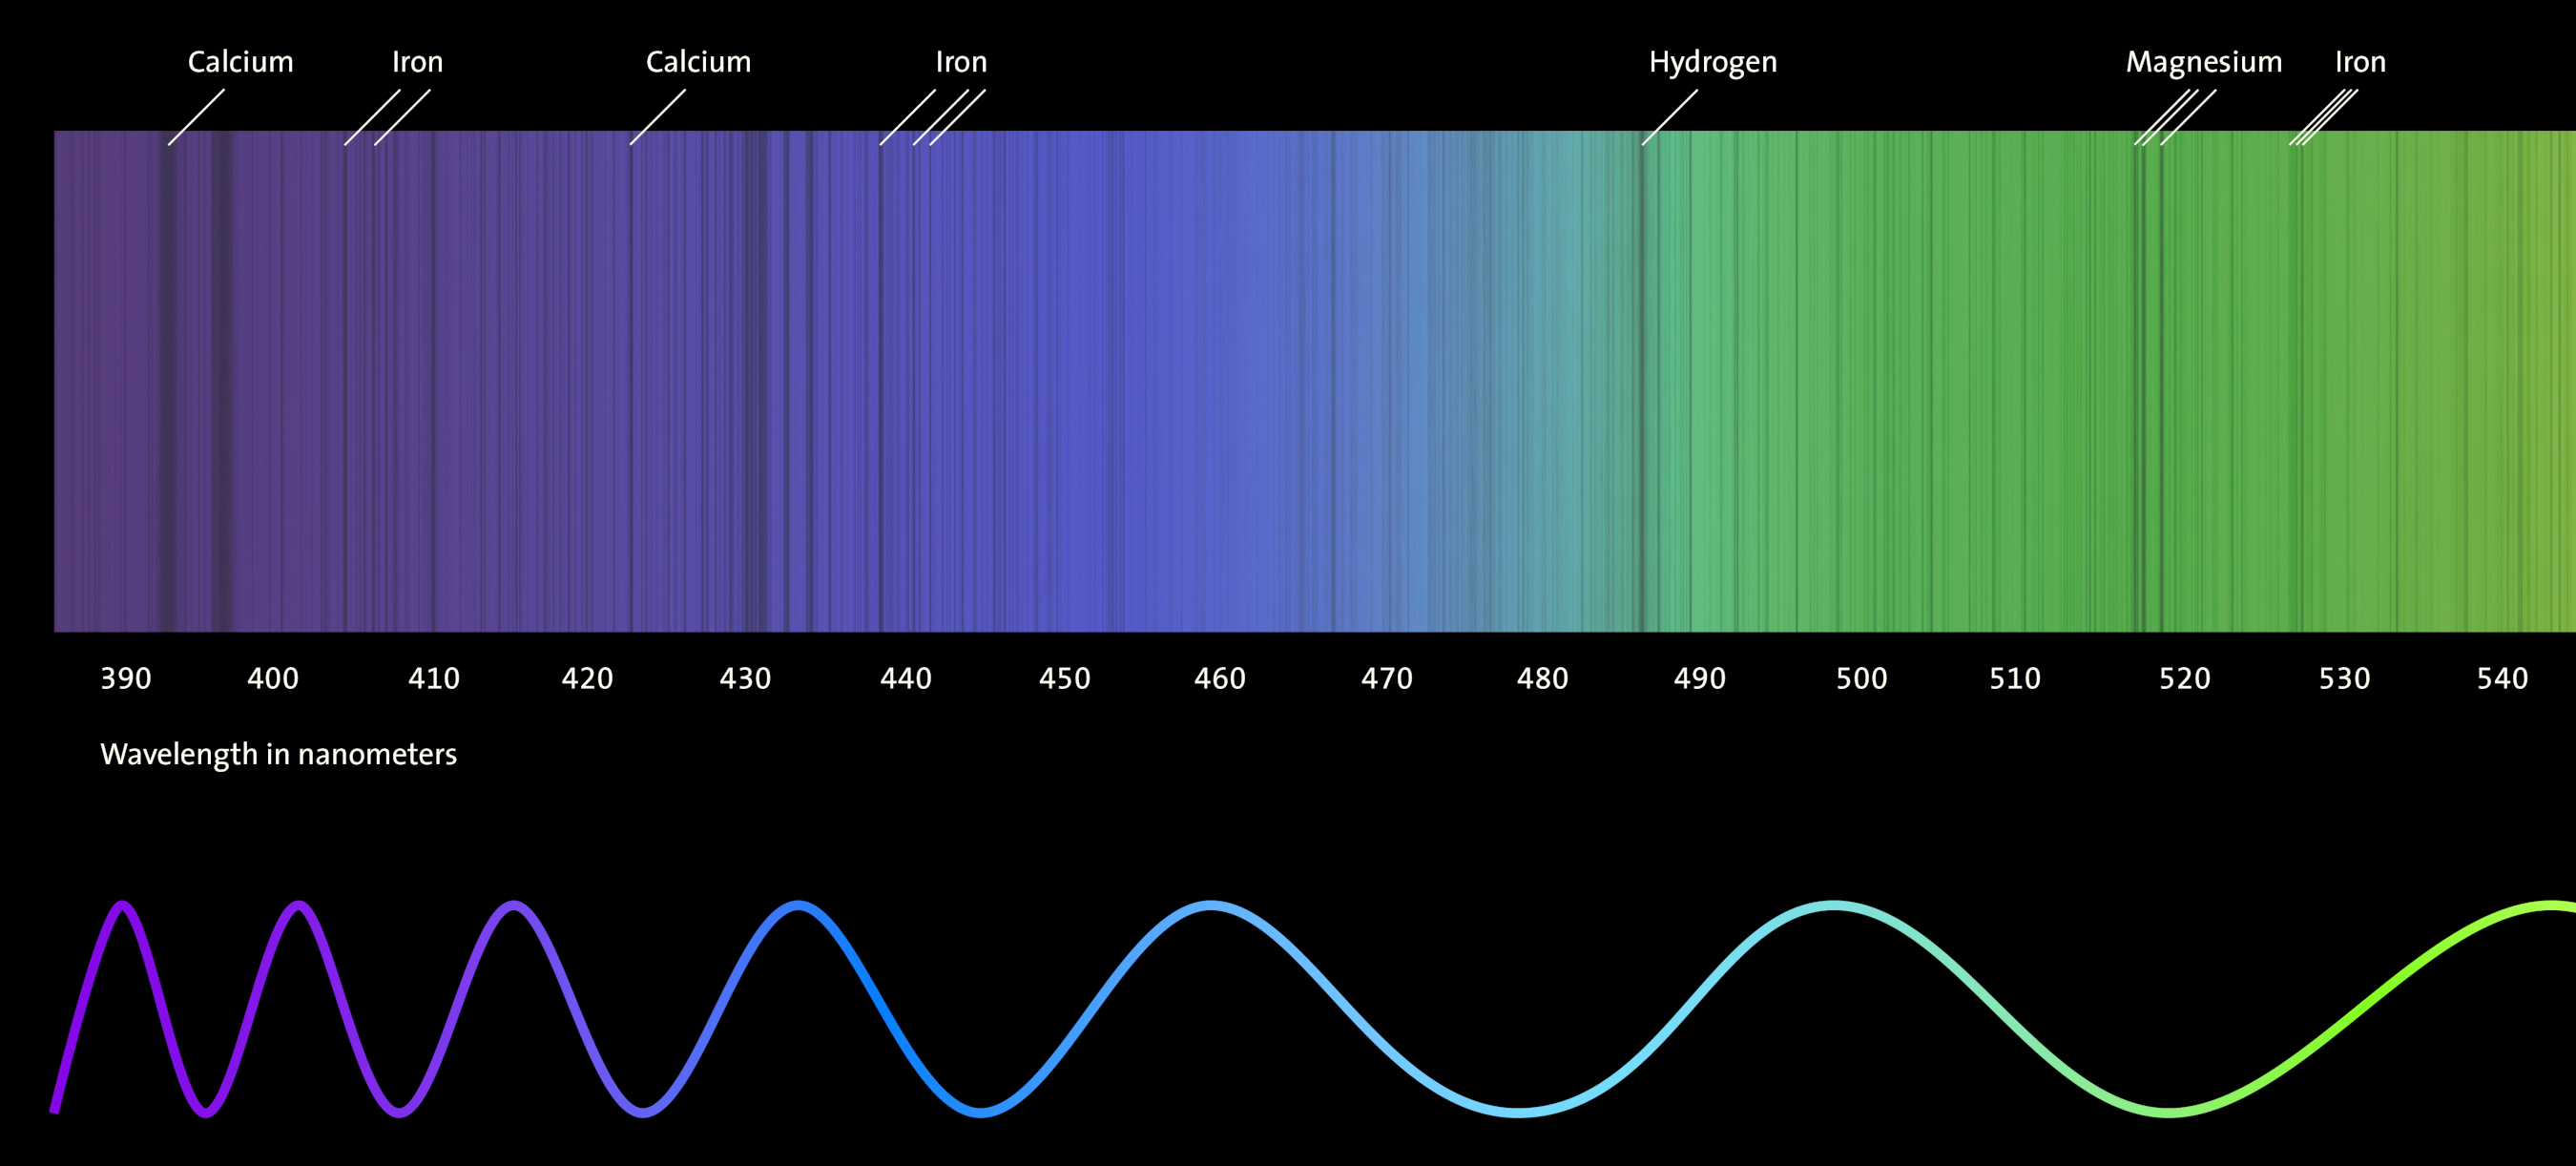
\includegraphics[width=0.48\linewidth]{images/griff_2.jpg}
    \hfill
    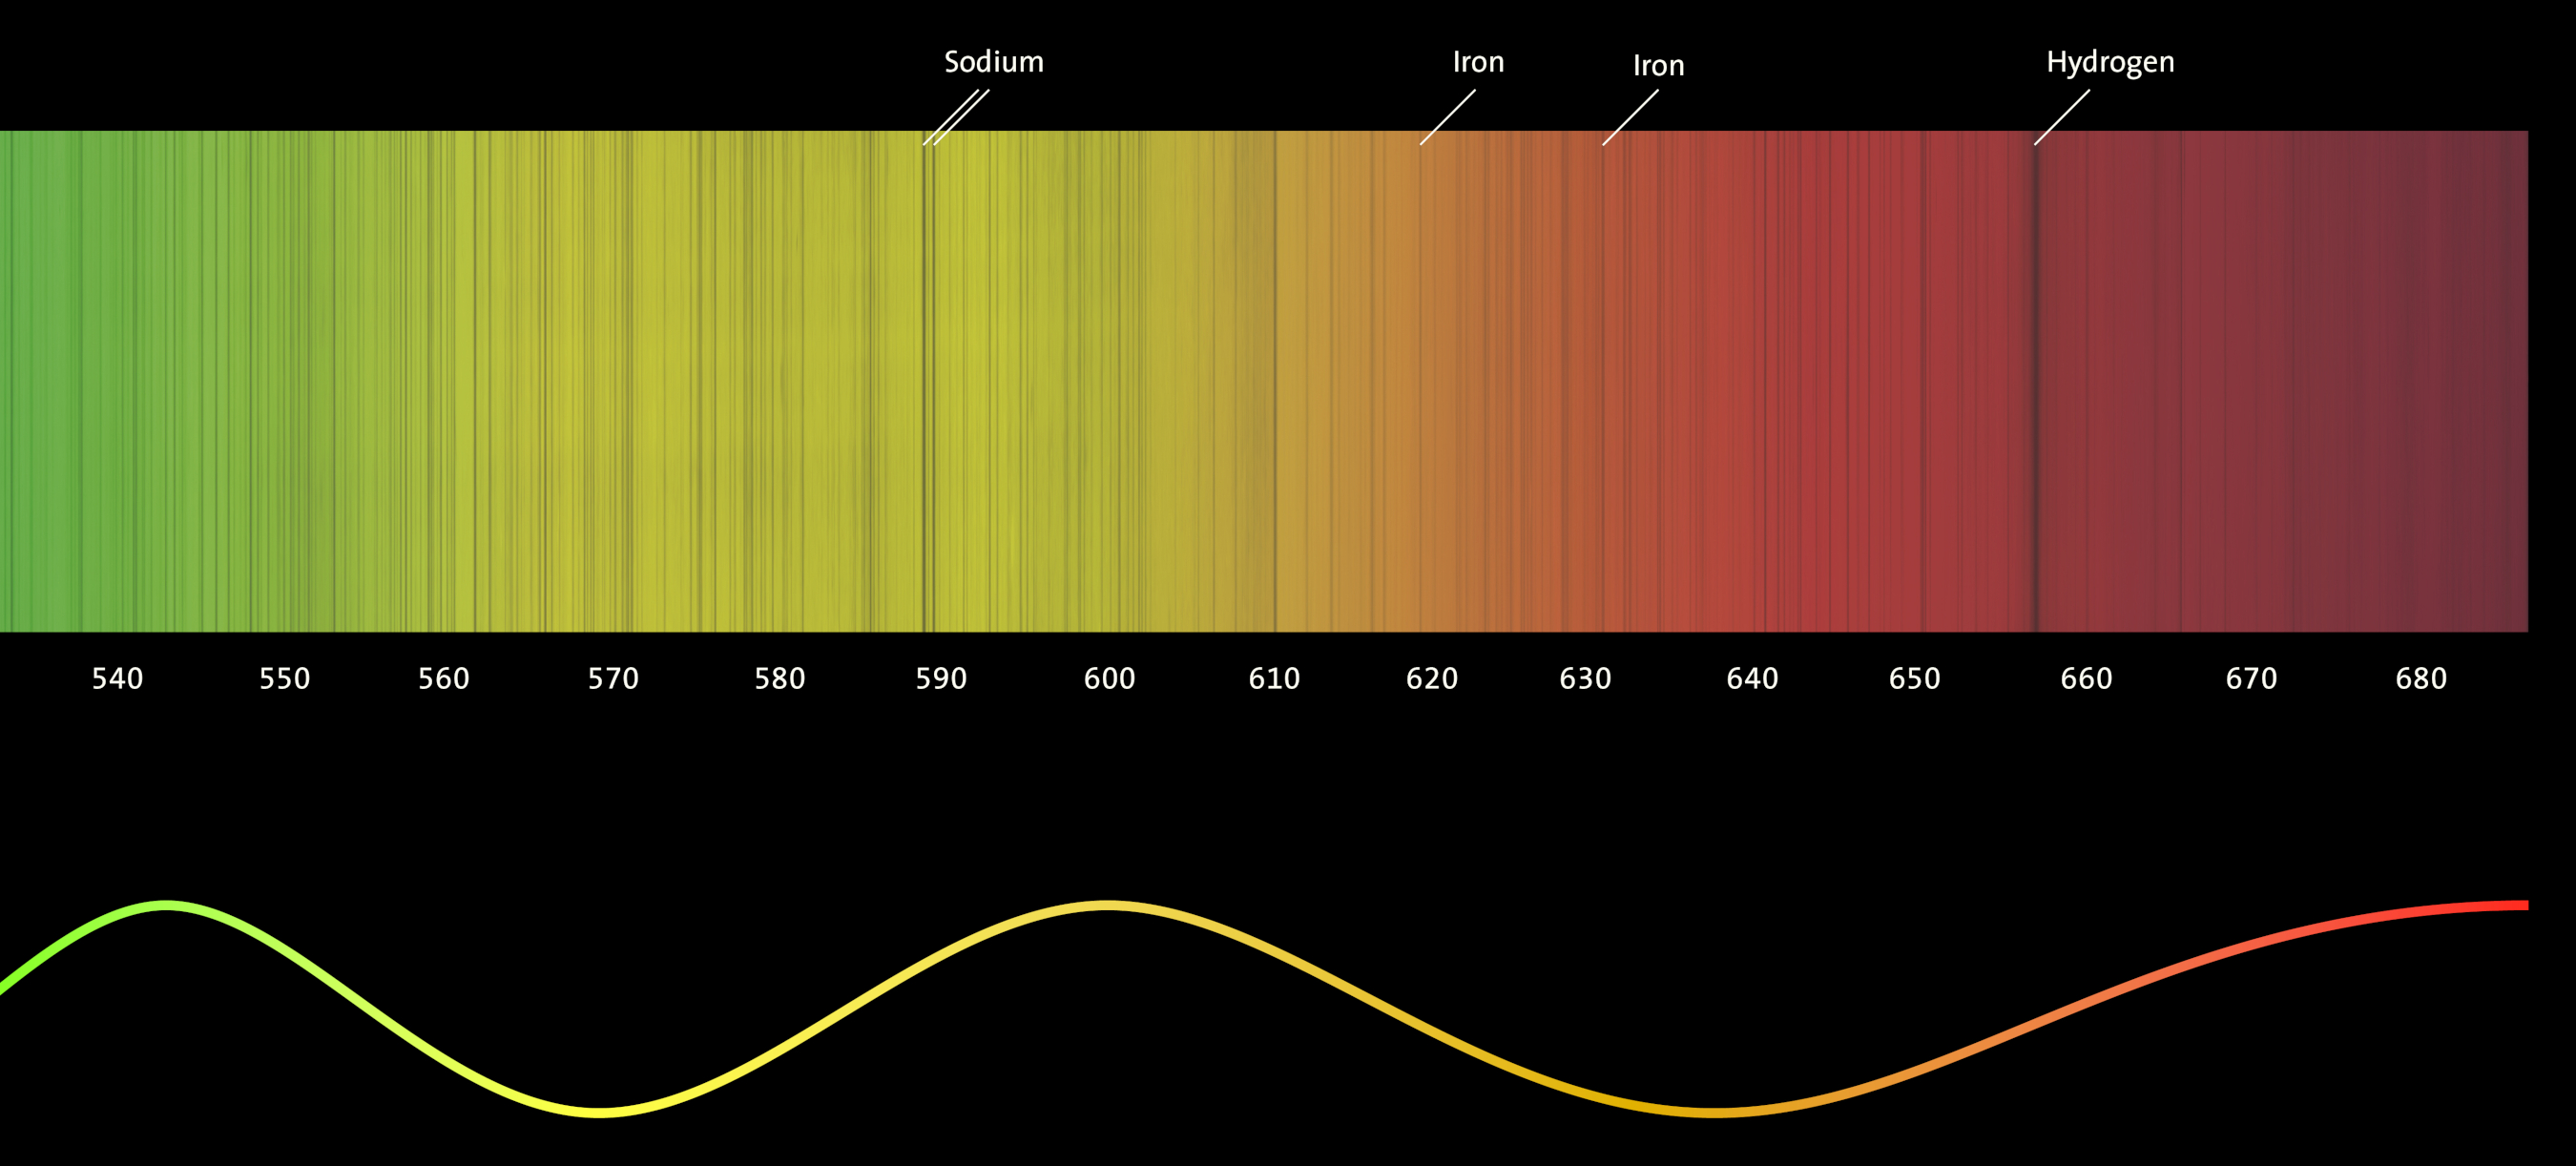
\includegraphics[width=0.48\linewidth]{images/griffith_lines.jpg}
    \caption{Spectroscopic images of the sun's light, courtesy of the Griffith Observatory.}
    \label{fig:spectroscopic-images}
\end{figure}

Although the importance of spectra is beyond question, their reliable computation is another matter (preface). In finite dimensions, we compute matrices, whose spectrum is the set of their eigenvalues. In particular, if $B \in \mathbb{C}^{nxn}$ then its spectrum is the following set of points:
\begin{equation} \label{matrix spec}
    \operatorname{Sp}(B) = \{z \in \mathbb{C}: \det (B-zI) = 0 \} = \{z \in \mathbb{C}: (B-zI)^{-1} \text{ does not exist} \},
\end{equation}
where $I$ denotes the identity matrix. 
% One might be tempted to think that this is a straightforward problem. However, as we will see, even for non-normal matrices, computed eigenvalues may be unreliable. 
In infinite dimensions, we consider a linear operator $A$ on a Hilbert space $H,$ whose spectrum is defined by the following set:
\begin{equation} \label{SpA}
    \operatorname{Sp}(A) = \{z \in \mathbb{C}: (A-zI)^{-1} \text{ does not exist as a bounded operator on } H \},
\end{equation}
where $I$ denotes the identity operator. The spectrum of a linear operator includes the set of eigenvalues of $A,$ but is generally much richer (Matt). This follows from the fact that in infinite dimensions there are more ways for $A-zI$ to fail to have a bounded inverse. As a result, new phenomena are present in the spectra of linear operators that make them much harder to reliably compute. To see this, consider the right-shift operator, 
\begin{equation}\label{right shift}
    A(x_1, x_2, \dots) = (0, x_1, x_2, \dots),
\end{equation}
that acts on a square-summable\footnote{Claiming that a sequence is `square-summable' is claiming that the sequence is in $l^2.$ The $l^2$ space consists of the space of sequences $(x_n)_{n\in \mathbb{N}}$  that satisfy $\sum_n x_n^2 < \infty.$} sequence of points, $(x_n)_{n\in \mathbb{N}}.$  This operator's spectrum is equal to the unit disc, but it has no eigenvalues\footnote{For more information on this example, see Appendix ?}.

The standard approach for computing the spectra of an infinite-dimensional operator is often refered to as the \textit{discretize-then-solve} approach. This approach consists of discretizing the operator with a finite-dimensional matrix, computing the spectrum of the discretized operator, and hoping that the spectrum of the discretized operator approaches the spectrum of the infinite-dimensional operator as the size of the discretization increases. Despite being a successful approach for many problems, it is fraught with difficulties. If the problem is not discretized very carefully, \textit{spectral pollution} can occur, where the discretized operator has eigenvalues that converge to something not in the spectrum of the infinite-dimensional operator (Patrick). Furthermore, the approach can suffer from \textit{spectral invisibility}, where discretizing the operator causes us to miss parts of the spectrum, even as the size of the discretization increases. Even if our discretization manages to avoid both spectral pollution and spectral invisibility, there remains a far more catastrophic limitation of the discretize-then-solve approach. In particular, since the spectra of infinite-dimensional operators may include more than just eigenvalues of finite multiplicity, there may be parts of the spectrum that we can never capture with the finite, discrete set of eigenvalues that results from discretization. 

These major pitfalls of the discretize-then-solve approach motivate the development of alternative methods for computing the spectra of infinite-dimensional operators. This challenge has been taken up by Matthew Colbrook at Cambridge. In recent work, Colbrook has proposed a new algorithm for computing the spectra of infinite-dimensional operators. Under certain conditions on the operator, this method yields a convergent approximation of the spectrum that captures the continuous components of the spectrum and does not suffer from spectral pollution or spectral invisibility. 
\begin{itemize}
    \item Quick overview of the algorithm
    \item Issues with it
    \item Our ideas 
\end{itemize}




% For example, if the range of $(A-zI)$ is not all of $H,$ $z \in \operatorname{Sp}(A)$ even if $z$ is not an eigenvalue of $A.$

% As a result, the study of spectra has a long and rich history. 
% Long before the development of modern spectral theory, humans observed that a stretched string does not produce just one sound, but a collection of related sounds (Matts forward). From these observations came the central thought that complicated motion may be understood through the combination of simpler oscillatory components. 
% Spectral theory in the modern sense, is often traced back to Fourier's solution of the the heat equation with series expansions, along with Euler and Lagrange'sstudy of eigenvectors in relation to rigid body motion (Matt, Preface). The field continued to be developed in the 19th century with contributions from scientists such as Cauchy, Cayley, Hermite, Liouville, Poincaré, Poisson, Rayleigh, Schwarz, Sturm, and Sylvestor (preface). In the 20th century, Hilbert's use of infinite matrices to study the eigenvalues of integral operators shaped much of the infinite-dimensional spectral theory considered today. Weyl extended the thoery to singular second-order ordinary differential equations (ODEs), von Neumann pioneered spectral theory for unbounded self-adjoint operators, and Riesz and Stone ...? 


\section{Motivations and  Project Goals}

\section{Main Contributions}
The examiners have suggested that a ``main contributions'' section in the introduction is really useful, so please ensure you have such a section! You can use this to explain what you believe are the main results of your work. If any of what you have done is novel, it can be helpful to highlight that here. If you have worked on an industrial project you could state how and why your results are useful to your industrial partner.

\section{Structure of the Dissertation}
It is common, although not compulsory, to end the introduction with a brief section explaining the structure of the dissertation. Often this goes along the lines of:
The remainder of the dissertation is structured as follows. In Chapter 2 we discuss blah blah. In Chapter 3 we blah blah. Finally in Chapter 4 we summarise the work we have done and suggest some areas for future research.

\section{Code Availability}
Here you may have a link to your GitHub repository (recommended but not mandatory). You can also make clear whether you have written code from scratch, or based it on other code, or had help from ChatGPT.

